\chapter{基础理论}
\section{复杂网络基本概念}
21世纪是复杂性和网络化的世纪。从20世纪七八十年代开始,在国际上形成了非线性科学和复杂性问题的研究热潮。尤其是20世纪90年代以来,
人类已经生活在一个充满各种各样复杂网络的世界中,许多复杂性问题都可以从复杂网络的角度去研究。
随着以互联网为代表的网络信息技术的迅速发展,人类社会已经迈入了复杂网络时代。人类的生活与生产活动越来越多地依赖于各种复杂网络系统安全可靠和有效的运行。
作为一个跨学科的新兴领域,“网络科学与工程”已经逐步形成并获得了迅猛发展。现在,许多发达国家的科学界和工程界都将这个新兴领域提上了国家科技发展规划的议事日程。
在中国,复杂系统包括复杂网络作为基础研究也已列入《国家中长期科学和技术发展规划纲要(2006-2020年)》。\par
网络科学与工程重点研究自然科学技术和社会政治经济中各种复杂系统微观性态与宏观现象之间的密切联系,特别是其网络结构的形成机理与演化方式、
结构模式与动态行为、运动规律与调控策略,以及多关联复杂系统在不同尺度下行为之间的相关性等。网络科学与工程融合了数学、统计物理、计算机科学及各类工程技术科学,
探索采用复杂系统自组织演化发展的思想去建立全新的理论和方法,其中的网络拓扑学拓展了人们对复杂系统的认识,而网络动力学则更深入地刻画了复杂系统的本质。
网络科学既是数学中经典图论和随机图论的自然延伸,也是系统科学和复杂性科学的创新发展。\par

图论是一种强有力的研究工具和研究方法。图(Graph)提供了一种用抽象的点和线表示各种实际网络的统一方法,因而也成为目前研究复杂网络的一种共同的语言。
下面我们给出图论的几个基本概念。
\subsection{图论的基本知识}
图是对系统中基本单元(称为节点)集合,以及每两个基本单元之间关系(边)集合之间关系的描述。图可以定义为一个三元组$G=(V,E,\phi)$
集合$V=\{v_1,v_2,…,v_n\}$称为节点集;
集合$E=\{e_1,e_2,…,e_m\}$称为边集;

$\phi$是边集E到节点集V的一个映射,称为关联函数。
V中的元素称为节点或顶点(node或vertex), E中的元素称为边、弧或连线(edge,arc或line),且E中的每条边em都有V的一对节点$(v_i,v_j)$与之对应。
用计算机分析实际网络的性质面临的第一个问题就是如何在计算机中表示一个网络。图的矩阵表示架起了图论与矩阵论之间的桥梁,通过这种表示方法就能借助于矩阵的理论和分析方法来研究图论中的问题。
邻接矩阵描述了节点与节点之间的邻接关系,通常会用一个方阵A来表示,方阵中的元素用$a_{ij}$表示。          

记$G=(V,E)$为一个非空图,其中$V$是其顶点集,$E$是边集。图中一点$v$的相邻点集记为$N(v)$,顶点的度是指与其相连的边的个数
记为$d(v)$,一个图的平均度定义为
\begin{equation}
    d(G):=\frac{1}{|V|} \sum_{v \in V} d(v)
\end{equation}
图$G$的一条路径是一个子图,其顶点集与边集描述了原图中某一点到另一点的一条通路。一个圈是指一个子图,描述了以某点为起始点与终止点
的一条非平凡路径。
一个含有$N$个节点、$M$个边的图$G$的密度定义$\rho$为
\begin{equation}
    \rho=\frac{M}{\frac{1}{2} N(N-1)}
\end{equation}
\begin{definition}
    如果非空图$G$中任意两顶点之间均有一条路相连,称图$G$为联通图。
\end{definition}
给定子图 $A,B \subseteq V$ 和 $X \subseteq V \cup E$,如果 $G$ 的每条 $A-B$ 路均包含 $X$ 中的一个顶点或一条边,
称在 $G$ 中 $X$ 分离 (separate) 集合 $A$ 和 $B$ 。
下面是图论中一个重要的定理。
\begin{theorem}
    设 $G=(V,E)$ 是一个图且 $A,B \subseteq V$ 。那么,在$G$ 中分离 $A$ 和 $B$ 的顶点的最小数目等于 $G$ 中互不
    相交的 $A-B$ 路的最大数目。
\end{theorem}
网络中节点的距离定义为连接这两个点的最小所经边数目。网络的平均长度定义为
\begin{equation}
    L=\frac{1}{\frac{1}{2} N(N-1)} \sum_{i \neq j} d_{i j}
\end{equation}
其中$d_{ij}$为节点$i,j$之间的距离。如果图本身并不联通,则只计算相连两点的距离的算术平均数。
一个图的直径$D$定义为任意两个节点之间距离的最大值。
\begin{definition}
    图中一个节点$i$的聚类系数$C_i$定义为
\begin{equation}
    C_i=\frac{E_i}{\left(k_i\left(k_i-1\right)\right) / 2}=\frac{2 E_i}{k_i\left(k_i-1\right)}
\end{equation}
其中$k_i$为该节点的度,$E_i$为其$k_i$个邻节点之间存在的边的数目。
还有一种聚类系数的几何定义,两个定义并不等价,一般会加以说明
\begin{equation}
    C_i=\frac{\text { 包含节点 } i \text { 的三角形的数目 }}{\text { 以节点 } i \text { 为中心的连通三元组的数目 }}
\end{equation}
\end{definition}
图的聚类系数定义为节点的聚类系数的均值
\begin{equation}
    C=\frac{1}{N} \sum_{i=1}^N C_i
\end{equation}
\subsection{规则网络}
如果系统中节点及其与边的关系是固定的,每个节点都有相同的度数,就可以用规则图来表示这个系统。这样的网络就称为规则网络。
常见的规则网络包括:全局耦合网络、最近邻耦合网络和星形耦合网络等。他们的结构示意图如下:
\begin{figure}[!htbp]
    \centering
    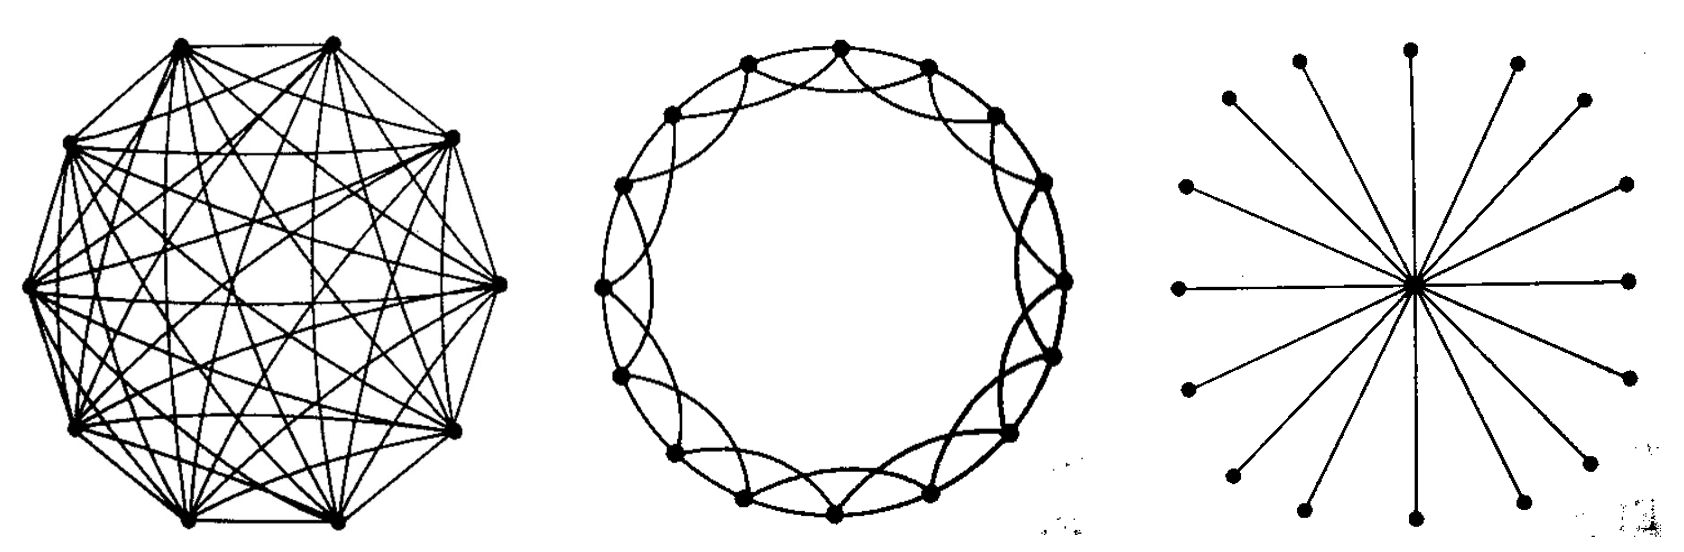
\includegraphics[width=0.8\textwidth]{guize.png}
    \caption{规则网络}
\end{figure}

\subsection{复杂网络}
系统是由相互作用和相互依赖的若干组成部分结合的具有特定功能的有机整体。从三个方面理解系统的概念:
     ①系统是由若干要素(部分)组成的。
     ②系统有一定的结构。
     ③系统有一定的功能。
     系统有如下的属性:
     集合性、相关性、层次性、整体性、涌现性、对环境的适应性
从图论意义上理解网络,网络是指由节点和连线构成的图。有时用带箭头的连线表示从一个节点到另一个节点存在的某种顺序关系。有时在节点或连线旁标出数值,称为点权或线权,有时不标任何数。
网络和系统通常是密切联系的,如果用节点表示系统的各个组成部分即系统的元素,两个节点之间的连线表示系统元素之间的相互作用,那么网络就为研究系统提供了一种新的描述方式。
一般认为复杂系统具有以下特征:非线性与动态性、非周期性和开放性、奇怪吸引性、结构自相似性(分形)。另外,复杂系统还具有突现性、不稳性、不确定性、不可预测性等特征。
复杂网络可以看作由一些具有独立特征的又与其他个体相互连接的节点的集合,每个个体可视为图中一个节点,节点间的相互连接视为图中的边。复杂网络包括两个层面:作为其连接拓扑结构的图和作为其状态和功能的系统。
\par 钱学森给出了复杂网络的一个较严格的定义:具有自组织、自相似、吸引子、小世界、无标度中部分或全部性质的网络称为复杂网络。
原则上说,任何包含大量组成单元(或子系统)的复杂系统,当我们把构成单元抽象成节点,单元之间的相互作用抽象为边时,都可以当作复杂网络来研究。

复杂网络是指不规则、度分布不均匀的网络模型,常见的复杂网络模型有全随机方式生成的ER随机图,在规则网络上进行修改的小世界模型。本节内容会给出
这几种的复杂网络模型的生成方法与其性质。
\subsubsection{ER随机图}
与完全规则网络相反的是完全随机网络。典型的模型是Erdös和Rényi于40多年前开始研究的ER随机图模型,其顶点采用完全随机连边的方式进行连接,它是一种完全随机图
,是随机性最强的图。下面我们首先给出具有固定次数连接独立两点的ER随机图$G(N,M)$的构造算法:\par 
\noindent(1) 初始化: 给定 $N$ 个节点和待添加的边数 $M$ 。\par
\noindent(2) 随机连边:\par
1) 随机选取一对没有边相连的不同的节点,并在这对节点之间添加一 条边。\par
2)重复步骤1),直至在 $M$ 对不同的节点对之间各添加了一条边。\par
然后给出以一定概率连接各独立顶点的ER 随机图 $G(N,p)$ 构造算法:\par
\noindent(1) 初始化: 给定 $N$ 个节点以及连边概率 $p \in[0,1]$ 。\par
\noindent(2) 随机连边:\par
1) 选择一对没有边相连的不同的节点。\par
2) 生成一个随机数 $r \in(0,1)$ 。\par
3) 如果 $r<p$,那么在这对节点之间添加一条边; 否则就不添加边。\par
4) 重复步骤1)-3),直至所有的节点对都被选择过一次。\par
对第二种$G(N,M)$进行性质分析。首先生成的随机图恰好具有 $M$ 条边的概率为
\begin{equation}
    P(M)=\left(\begin{array}{c}
    C^2_N \\
    M
    \end{array}\right) p^M(1-p)\left(\begin{array}{c}
    N \\
    2
    \end{array}\right)^{-M}
\end{equation}
其中,$C^2_N=\left(\begin{array}{c}
    N \\
    2
    \end{array}\right)$,
$\left(\begin{array}{c}
    C^2_N \\
    M
    \end{array}\right)$表示具有 $N$ 个节点和 $M$ 条边的简单图的数量,
    $p^M(1-p)^{C^2_N-M}$ 
表示有 $M$ 对节点之间添加了边, $C^2_N-M$ 对节点之间没有添加边。
边数分布的平均值为:
\begin{equation}
    \langle M\rangle=\sum_{n=0}^{C^2_N} M P(M)=\left(\begin{array}{l}
    N \\
    2
    \end{array}\right) p=p \frac{N(N-1)}{2}
    \end{equation}
边数分布的方差:
\begin{equation}
    \sigma_M^2=\left\langle M^2\right\rangle-\langle M\rangle^2=p(1-p) \frac{N(N-1)}{2}
\end{equation}
$G(N,M)$中节点度的概率分布符合泊松分布。
\begin{equation}
    P(k)=\left(\begin{array}{c}
    N-1 \\
    k
    \end{array}\right) p^k(1-p)^{N-1-k}
\end{equation}
根据概率统计中的内容,其期望与方差分别为
\begin{equation}
    \langle k\rangle=p(N-1)
\end{equation}
\begin{equation}
    \sigma_k^2=p(1-p)(N-1)
\end{equation}
由于两个节点之间不论是否具有共同的邻居节点,共连接概率均为$p$,所以聚类系数为
\begin{equation}
    C=p=\langle k\rangle /(N-1)
\end{equation}
\subsubsection{WS小世界模型}
WS小世界模型是通过在规则图上做带有随机性的更改形成的。下面给出WS模型构建算法如下:\par
\noindent(1) 从规则图开始: 给定一个含有 $N$ 个点的环状最近邻耦合网络,其中 每个节点都与它左右相邻的各 $K / 2$ 个节点相连,$K$ 是偶数。\par
\noindent(2) 随机化重连: 以概率 $p$ 随机地重新连接网络中原有的每条边,即把 每条边的一个端点保持不变,另一个端点改取为网络中随机选择的一个节点。
其中规定不得有重边和自环。\par
\begin{figure}[!htbp]
    \centering
    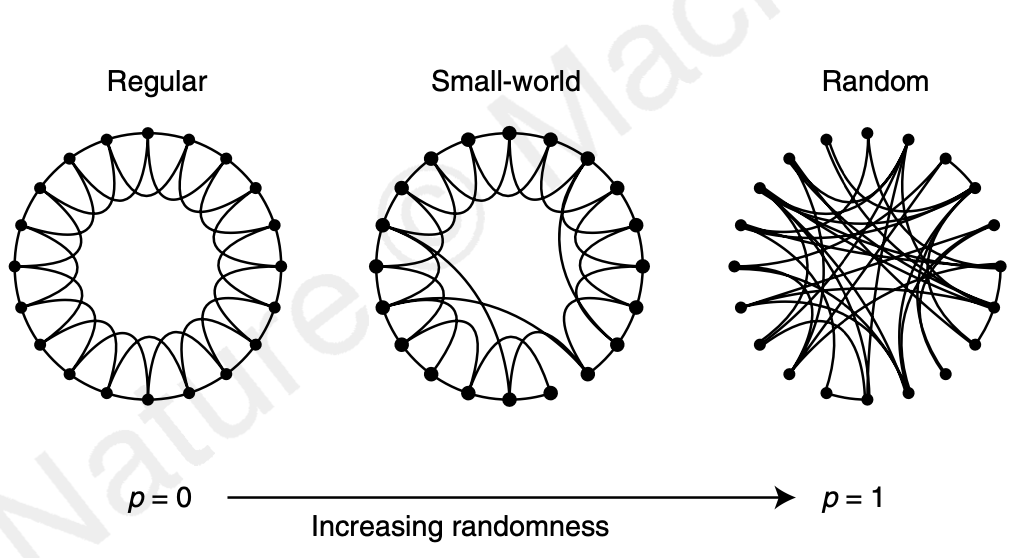
\includegraphics[width=0.8\textwidth]{wsp.png}
    \caption{WS随机网络的构造}
\end{figure}
可以看出,$p=0$时是完全规则的网络,$p=1$时是完全随机的网络。WS模型的聚类系数与平均路径长度是关于重连概率$p$的函数,
其关系如下图\par
\begin{figure}[!htbp]
    \centering
    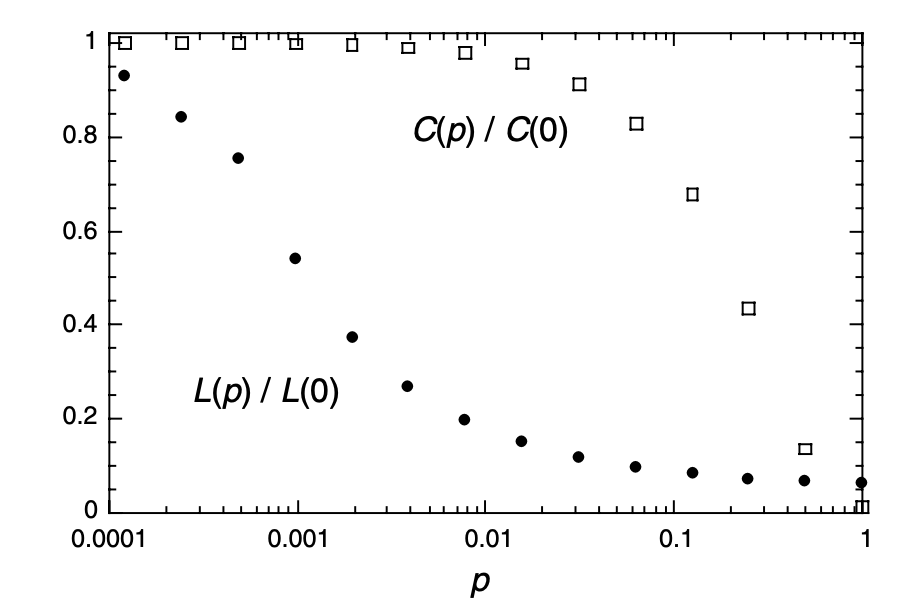
\includegraphics[width=0.8\textwidth]{WS.png}
    \caption{WS随机网络的聚类系数与重连概率}
\end{figure}
WS模型的聚类系数的估计如下
\begin{equation}
    \begin{aligned}
    \tilde{C}_{W S}(p) & \triangleq \frac{M_0(1-p)^3+O(1 / N)}{K(K-1) / 2} \\
    & =\frac{3 K(K-2) / 8}{K(K-1) / 2}(1-p)^3+O(1 / N) \\
    & =\frac{3(K-2)}{4(K-1)}(1-p)^3+O(1 / N) \\
    & =C_{n c}(1-p)^3+O(1 / N)
    \end{aligned}
\end{equation}\par
下面来研究WS模型的度分布,在 $p>0$ 时,每个节点仍与顺时针方向的 $K / 2$ 条原有的边相连,即每个节点的度至少为 $K / 2$ 。
 为此,记节点 $i$ 的度为 $k_i=s_i+K / 2$。 $s_i$ 又可分为两部分: 
 $s_i=s_i^1+s_i^2$,$s_i^1$ 表示在原有的与节点 $i$ 相连的逆时针方向的 $K / 2$ 条边中保持不变的边的数目,
 其中每条边不变的概率为 $1-p ; s_i^2$ 表示通过随机重连机制连接节点 $i$ 上的长程边,
 每条这样的边的概率 为 $p / N$ 。有
 \begin{equation}
    \begin{gathered}
    P_1\left(s_i^1\right)=\left(\begin{array}{c}
    K / 2 \\
    s_i^1
    \end{array}\right)(1-p)^{s_i^{1}} p^{K / 2-s_i^1}\\
    P_2\left(s_i^2\right) \simeq \frac{(p K / 2)^{s_i^2}}{\left(s_i^2\right) !} \mathrm{e}^{-\rho K / 2}\text { 当 } N \text { 充分大时. }
    \end{gathered}
\end{equation}
对于任一度为 $k \geqslant K / 2$ 的节点,$s_i^1 \in[0,\min (k-K / 2,K / 2)]$ 。
当$k<K/2$时,$P(k)=0$,当 $k \geqslant$ $K / 2$ 时
\begin{equation}
    P(k)=\sum_{n=0}^{\min (k-K / 2,K / 2)}\left(\begin{array}{c}
    K / 2 \\
    n
    \end{array}\right)(1-p)^n p^{K / 2-n} \frac{(p K / 2)^{k-(K / 2)-n}}{(k-(K / 2)-n) !} \mathrm{e}^{-p K / 2}
\end{equation}
\subsubsection{NW小世界模型}
NW小世界模型是通过在规则图上有随机性的增加长程边形成的,相比WS模型,这是一种更常见的小世界模型。
下面给出NW模型构建算法如下\par
\noindent(1) 从规则图开始: 给定一个含有 $N$ 个节点的环状最近邻耦合网络,其中每个节点都与它左右相邻的各 $K / 2$ 个节点相连,$K$ 是偶数。\par
\noindent(2) 随机化加边: 以概率 $p$ 在随机选取的 $NK / 2$ 对节点之间添加边,其中 规定不得有重边和自环。\par
首先讨论NW模型的聚类系数,NW模型的聚类系数采用几何聚类系数来讨论,$p=0$ 时,网络中的三角形数量为 
$\frac{1}{4} N K\left(\frac{1}{2} K-1\right)$。$ p>0$ 时,
现在我们需要计算在添加了长程边之后新增加的三角形的数量。 网络中长程边的平均数为 $\frac{1}{2} N K p$,
这些边可以在 $\frac{1}{2} N(N-1)$ 个点对之间添加,每一对节点之间有长程边相连的概率为
\begin{equation}
    \frac{\frac{1}{2} N K p}{\frac{1}{2} N(N-1)}=\frac{K p}{N-1} \approx \frac{K p}{N}
 \end{equation}
 包含一条长程边的三角形数量可以近似为一个与$N$无关的常数:
 \begin{equation}
    N \times \frac{K p}{N}=K p
\end{equation}
当网络规模趋于无穷时,这一常数与最近邻网络的三角形数量相比是可以忽略不计的。因此,对于 $0 \leqslant p \ll 1$ 
模型中的三角形的数量近似为 $\frac{1}{4} N K\left(\frac{1}{2} K-1\right) $
每条长程边都可以与$N$条边的两个端点之一形成连通三元组,因此包含一条长程边的连通三元组的平均数量为
\begin{equation}
    \frac{1}{2} N K p \times K \times 2=N K^2 p
\end{equation}
如果一个节点与 $m>1$ 条长程边相连,那么从中任选两条长程边就构成一个 连通三元组,共有 $\frac{1}{2} m(m-1)$ 种可能。
平均一个节点与 $K p$ 条长程边相连,因此 网络中以一个节点为中心的包含两条长程边的连通三元组数量的均值为
\begin{equation}
    N \times \frac{1}{2} K p(K p-1) \approx \frac{1}{2} N K^2 p^2
\end{equation}
因此,NW模型中总的连通三元组的数量的均值为
\begin{equation}
    \frac{1}{2} N K(K-1)+N K^2 p+\frac{1}{2} N K^2 p^2
\end{equation}
综上所述,当$0 \leqslant p<1$时,NW小世界网络模型的聚类系数的估计值为
\begin{equation}
    \begin{aligned}
    \tilde{C}_{N W}(p) & =\frac{3 \times \frac{1}{4} N K\left(\frac{1}{2} K-1\right)}{\frac{1}{2} N K(K-1)+N K^2 p+\frac{1}{2} N K^2 p^2} \\
    & =\frac{3(K-2)}{4(K-1)+4 K p(p+2)} 
    \end{aligned}
\end{equation}
小世界模型的平均路径长度具有如下形式
\begin{equation}
    L=\frac{N}{K} f(N K p)
\end{equation}
$f(x)$被称为普适标度函数,NW模型的平均路径长度有如下近似
\begin{equation}
    f(x)=\frac{2}{\sqrt{x^2+4 x}} \operatorname{artanh} \sqrt{\frac{x}{x+4}}
\end{equation}
在$x$远大于1时,可以简化为
\begin{equation}
    f(x) \simeq \frac{1}{\sqrt{x^2+4 x}} \ln \frac{\sqrt{1+4 / x}+1}{\sqrt{1+4 / x}-1} \simeq \frac{\ln x}{x},\quad x>>1
\end{equation}
将$f(x)$代入,最后得出
\begin{equation}
    L=\frac{\ln (N K p)}{K^2 p},\quad N K p>>1
\end{equation}
由图看出,这种近似效果优异。\par
\begin{figure}[!htbp]
    \centering
    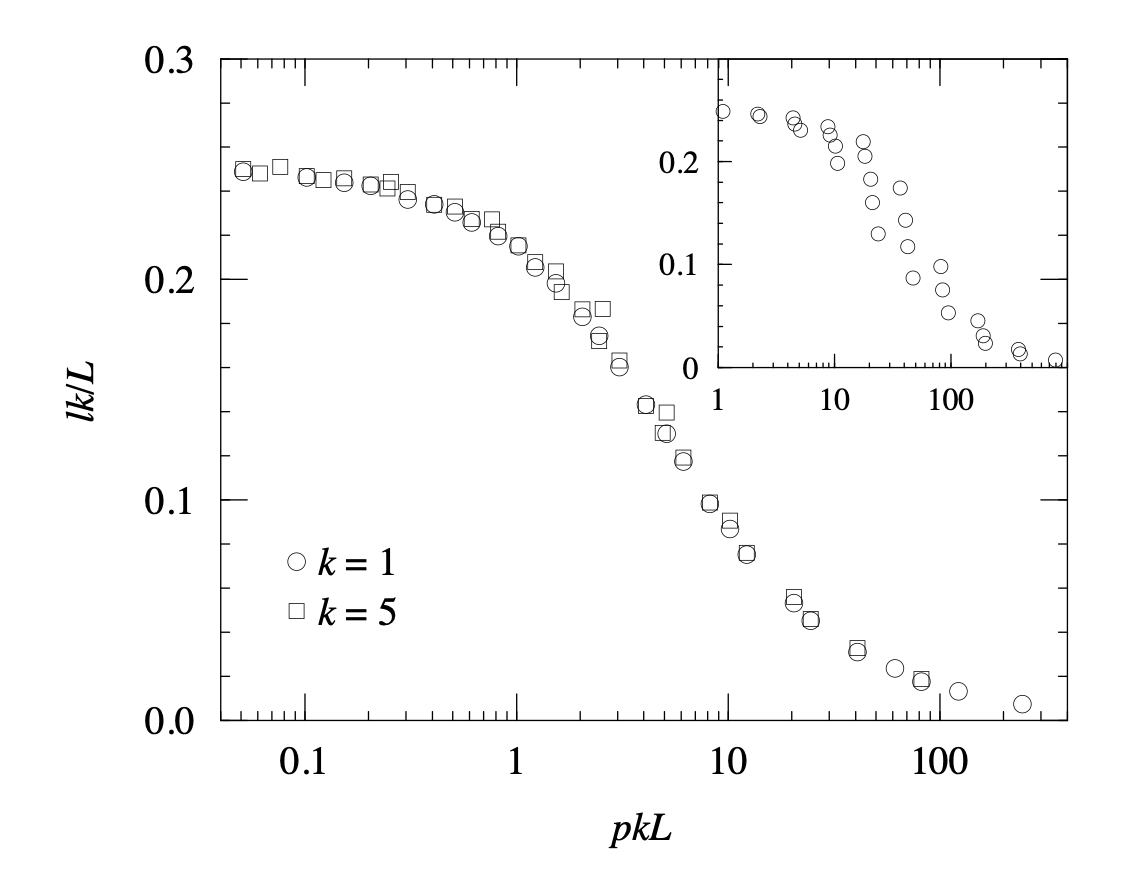
\includegraphics[width=0.8\textwidth]{NW1.png}
    \caption{NW随机网络的平均路径长度}
\end{figure}
下面讨论度分布,由于每对节点之间有边相连的概率为 $Kp/(N-1)$,因此
\begin{equation}
    P(k)=\left(\begin{array}{l}
    N-1 \\
    k-K
    \end{array}\right)\left[\frac{K p}{N-1}\right]^{k-K}\left[1-\frac{K p}{N-1}\right]^{N-1-k+K}
\end{equation}
NW模型中长程边的平均数为 $\frac{1}{2} N K p$,涉及的端点数目为 $N K p$ 。
因此,网络中长程边的数量为 $K p$,
即 $\langle k-K\rangle=K p$ 。当网络中节点数 $N$ 充分大时,可近似写为泊松分布:
\begin{equation}
    P(k)=\frac{(K p)^{k-K}}{(k-K) !} \mathrm{e}^{-K_p}
\end{equation}
\section{非线性系统的稳定性和混沌}
在刘慈欣的著作《三体》中提到了一个经典的天体物理问题——三体问题,这个问题的一个重要特点是三体系统的不稳定性,即在微小扰动的影响下,
依托于一定时间内已知的位置与运动信息预测出将来的位置具有很大的变化。现实中很难把握系统中全部的微信息,例如一个原子的微小扰动几乎是
难以描述的,如果模型自身对这种微小差异敏感度极高,那意味着这个系统几乎没有可以预测的可能性,预测出的结果与现实差异会随着时间轴指数级放大。
衡量非线性系统的稳定性研究主要由李雅普诺夫稳定性入手。
\subsection{非线性系统的稳定性}
考虑自治系统
\begin{equation}
    \dot{x}=f(x)
\end{equation}
其中 $,f: D \rightarrow R^n$ 是从定义域 $D \subset R^n$ 到 $R^n$ 上的局部利普希茨映射。
假定 $\bar{x} \in D$ 是其平衡点,即 $f(\bar{x})=0$ 。不失一般性,所有定义和定理都是对平衡点在 $R^n$ 上的原点,
即 $\bar{x}=0$ 时的情况而言。因为经过变量代换总可以把平衡点变换为原点。假设 $\bar{x} \neq 0$,经 $y=x-\bar{x}$ 变换后,$y$ 的
导数为
\begin{equation}
    \dot{y}=\dot{x}=f(x)=f(y+\bar{x}) \stackrel{\text { def }}{=} g(y),g(0)=0
\end{equation}
对于变量$y$,系统在原点有平衡点。
\begin{definition}
    对于平衡点$x=0$,如果对于每个 $\varepsilon>0$,都存在 $\delta=\delta(\varepsilon)>0$, 满足
    \begin{equation}
        \|x(0)\|<\delta \Rightarrow\|x(t)\|<\varepsilon,\quad \forall t \geqslant 0
    \end{equation}
    则该平衡,点是稳定的。
    如果稳定,且可选择适当的 $\delta$, 满足
    \begin{equation}
        \|x(0)\|<\delta \Rightarrow \lim _{t \rightarrow \infty} x(t)=0
    \end{equation}
    则该平衡,点是渐近稳定的。
\end{definition}
下面的李雅普诺夫稳定性定理是判断平衡点稳定的重要方法,它能够用某些其他函数代替能量以确定平衡点的稳定性。
设 $V: D \rightarrow R$ 是连续可微函数,$\dot{V}(x)$是$V(x)$沿方程轨线的导数。即
\begin{equation}
    \begin{aligned}
    \dot{V}(x) & =\sum_{i=1}^n \frac{\partial V}{\partial x_i} \dot{x}_i=\sum_{i=1}^n \frac{\partial V}{\partial x_i} f_i(x) \\
    & =\left[\begin{array}{llll}
    \frac{\partial V}{\partial x_1},& \frac{\partial V}{\partial x_2},& \cdots,& \frac{\partial V}{\partial x_n}
    \end{array}\right]\left[\begin{array}{c}
    f_1(x) \\
    f_2(x) \\
    \vdots \\
    f_n(x)
    \end{array}\right]=\frac{\partial V}{\partial x} f(x)
    \end{aligned}
\end{equation}
\begin{theorem}
    设 $x=0$ 是方程的一个平衡点,$D \subset R^n$ 是包含原点的定义域。设 $V: D \rightarrow R$ 是连续可微函数,如果
    \begin{equation}
        \begin{array}{lll}
        V(0)=0,& V(x)>0 & \text { 在 } D-\{0\} \text { 内 } \\
        & \dot{V}(x) \leqslant 0 & \text { 在 } D \text { 内 }
        \end{array}
    \end{equation}
    那么,原点 $x=0$ 是稳定的。此外,如果
    \begin{equation}
        \dot{V}(x)<0 \quad \text { 在 } D-\{0\} \text { 内 }
    \end{equation}
    那么,原点 $x=0$ 是渐近稳定的。
\end{theorem}
满足式(2.33)的连续可微函数 $V(x)$ 称为李雅普诺夫函数。对于某个 $c>0$,曲面 $V(x)=c$ 称为李雅普诺夫面或等位面。
下面是Chetaev定理,用于确定非稳定平衡点的不稳定性。
\begin{theorem}
    设 $x=0$ 是方程 $(4.1)$ 的平衡点。设 $V: D \rightarrow R$ 是连续可微函数,满足 $V(0)=0$,
    且对于任意小 $\left\|x_0\right\|$ 的某一点 $x_0$,有 $V\left(x_0\right)>0$ 。定义集合 $U=\left\{x \in B_r \mid V(x)>0\right\}$,
    并假设在 $U$ 内有 $\dot{V}(x)>0$,那么 $x=0$ 就是非稳定平衡点。
\end{theorem}
接下来讨论非线性系统线性化的方法,定义线性系统
\begin{equation}
    \dot{x}=A x
\end{equation}
该系统在原点处有一个平衡点,当且仅当 $\operatorname{det}(A) \neq 0$ 时,该平衡点是孤立的。
如果 $\operatorname{det}(A)=0$,则矩阵 $A$ 有一个非平凡零空间。 $A$ 的零空间内的每一点都是系统的平衡点,进而系统有一个平衡点子空间。
线性系统不可能有多个孤立的平衡点, 因为如果 $\bar{x}_1$ 和 $\bar{x}_2$ 是系统的两个平衡点, 那么连接 $\bar{x}_1$ 和 $\bar{x}_2$ 
两点的直线上的每一点都是系统的平衡点。原点的稳定性质由矩阵 $A$ 的特征值位置决定。对于给定的初始状态 $x(0)$,系统的解为
\begin{equation}
    x(t)=\exp (A t) x(0)
\end{equation}
转换为若尔当标准型
\begin{equation}
    P^{-1} A P=J=\operatorname{diag}\left[J_1,J_2,\cdots,J_r\right]
\end{equation}
\begin{equation}
    J_i=\left[\begin{array}{cccccc}
    \lambda_i & 1 & 0 & \ldots & \ldots & 0 \\
    0 & \lambda_i & 1 & 0 & \ldots & 0 \\
    \vdots & & \ddots & & & \vdots \\
    \vdots & & & \ddots & & 0 \\
    \vdots & & & & \ddots & 1 \\
    0 & \ldots & \ldots & \ldots & 0 & \lambda_i
    \end{array}\right]_{m \times m}
\end{equation}
因此
\begin{equation}
    \exp (A t)=P \exp (J t) P^{-1}=\sum_{i=1}^r \sum_{k=1}^{m_i} t^{k-1} \exp \left(\lambda_i t\right) R_{i k}
\end{equation}
\begin{theorem}
    当且仅当 $A$ 的所有特征值都满足 $\operatorname{Re} \lambda_i \leqslant 0$,对于每个 $\operatorname{Re} \lambda_i=0$,
    代数重数 $q_i \geqslant 2$ 的特征值满足 $\operatorname{rank}\left(A-\lambda_i I\right)=n-q_i$ 时
    ($n$ 为 $x$ 的维数),方程 $\dot{x}=A x$ 的平衡点 $x=0$ 是稳定的。 
    当且仅当 $A$ 的所有特征值满足 $\operatorname{Re} \lambda_i<0$ 时,平衡点 $x=0$ 是全局渐近稳定的。
\end{theorem}
回到非线性系统(2.29),$f: D \rightarrow R^n$ 是从 $D \subset R^n$ 到 $R^n$ 的连续可微映射。
假设原点 $x=0$ 在 $D$ 内,且为系统的一个 平衡点,即 $f(0)=0$ 。根据均值定理
\begin{equation}
    f_i(x)=f_i(0)+\frac{\partial f_i}{\partial x}\left(z_i\right) x
\end{equation}
其中 $z_i$ 是连接 $x$ 与原点之间的线段上的一点。由于$f(0)=0$
\begin{equation}
    f_i(x)=\frac{\partial f_i}{\partial x}\left(z_i\right) x=\frac{\partial f_i}{\partial x}(0) x+\left[\frac{\partial f_i}{\partial x}\left(z_i\right)-\frac{\partial f_i}{\partial x}(0)\right] x
\end{equation}
所以
\begin{equation}
    f(x)=A x+g(x)
\end{equation}
其中
\begin{equation}
    A=\frac{\partial f}{\partial x}(0),\quad g_i(x)=\left[\frac{\partial f_i}{\partial x}\left(z_i\right)-\frac{\partial f_i}{\partial x}(0)\right] x
\end{equation}
并且
\begin{equation}
    \left|g_i(x)\right| \leqslant\left\|\frac{\partial f_i}{\partial x}\left(z_i\right)-\frac{\partial f_i}{\partial x}(0)\right\|\|x\|
\end{equation}
\begin{equation}
    \frac{\|g(x)\|}{\|x\|} \rightarrow 0 \text {,当 }\|x\| \rightarrow 0
\end{equation}
这就是说在原点的一个小邻域内,可以用对系统在原点的线性化方程
\begin{equation}
    \dot{x}=A x,\quad \text { 其中 } A=\frac{\partial f}{\partial x}(0)
\end{equation}
下面定理指出当原点是非线性系统的平衡点时,其稳定性可以通过研究线性系统在该平衡点的稳定性得出。
\begin{theorem}
    设 $x=0$是非线性系统$\quad \dot{x}=f(x)$的一个平衡点,其中 $f: D \rightarrow R^n$ 是连续可微的,
    且 $D$ 为原点的一个邻域。设
    \begin{equation}
        A=\left.\frac{\partial f}{\partial x}(x)\right|_{x=0}
    \end{equation}
    如果 $A$ 的所有特征值都满足 $\operatorname{Re} \lambda_i<0$,则原点是渐近稳定的。如果 $A$ 至少有一个特征值满足 $\operatorname{Re} \lambda_i>0$,则原点是不稳定的。
\end{theorem}
\subsection{混沌基本理论}
\subsubsection{混沌定义}
从牛顿力学创立之初,人们就坚信 Laplace 确定论思想,即对确定性动力系统 施加确定性输入,将得到确定性的输出. 这一结论对于线性系统是正确的,但对于非线性系统,
则可能出现一种不可预测的、类随机的运动,即混沌 (chaos). 由于混沌的奇异性、复杂性尚未被彻底揭示,其定义至今尚不统一。首先来介绍Li-Yorke 定义。
\begin{theorem}(Li-Yorke)
    若 $f(x)$ 为 $[a, b]$ 上的连续自映射,且 $f(x)$ 有 3 周期点,则 $\forall n \in \mathbb{Z}^{+}, f(x)$ 存在 $n$ 周期点。
\end{theorem}
\begin{definition}(Li-Yorke)
区间 $I$ 上的连续自映射 $f(x)$ 具有混沌现象,若其满足:\par
(1) $f$ 的周期点的周期无上界,\par
(2) $I$ 上存在不可数子集 $S$,有\par
(i) 对任意 $x, y \in S, x \neq y$ 时,$\lim _{n \rightarrow \infty} \sup \left|f^n(x)-f^n(y)\right|>0$;\par
(ii) 对任意 $x, y \in S, \lim _{n \rightarrow \infty} \inf \left|f^n(x)-f^n(y)\right|=0$;\par
(iii) 对任意 $x \in S$ 和 $f$ 的任意周期点 $y$,有 $\lim _{n \rightarrow \infty} \sup \left|f^n(x)-f^n(y)\right|>0$。
\end{definition}
由定义可知:闭区间 $I$ 上的连续函数 $f (x)$,若存在 3 周期点,则必存在任意正整数周期点, 即存在混沌现象。定义中,条件 (i)、(ii) 表明子集中的点 $x$ 与 $y$ 相当分散又相当集中,
条件 (iii) 意味着子集不会趋近于任意周期点. Li-Yorke 定义准确刻画了混沌运动的三个重要特征:
(1) 存在不可数无穷多稳定非周期轨道;(2) 至少存在一个不稳定的非周期轨道;(3) 存在可数无穷多稳定周期轨道。\par
接下来是下一种定义混沌的方法——Devaney 混沌定义。
\begin{definition}(Devaney)
设 $V$ 是一度量空间,称映射 $f: V \rightarrow V$ 为混沌的,若其满足:\par
(1) 初值敏感性, $\exists \delta>0, \forall \varepsilon>0$ 与 $\forall x \in V, \exists y \in O_x(\varepsilon)$ 与 $n \in \mathbb{N}$, s.t. $d\left(f^n(x), f^n(y)\right)>\delta$;\par
(2) 拓扑传递性, 对 $V$ 上任意开集 $X, Y, \exists k>0, f^k(X) \cap Y \neq \varnothing$ (如映射有稠 轨道, 则其显然是拓扑传递的);\par
(3) $f$ 的周期点集在 $V$ 中稠密。
\end{definition}

Devaney 定义从另外的角度刻画了混沌的重要特征, 包括:(1) 初值敏感性:任意两点 x,y 即使非常靠拢,它们之间的距离在 $f$ 作用多次
后都将扩大到一定的程度, 任意微小的初始误差,经多次迭代后都将导致计算 $f$ 轨 道的失败;(2) 拓扑传递性:在 $f $的作用下, 任意点的邻域将遍及整个度量空间 V,
表明$f$ 无法分解为在 $f$ 下互不相影响的两个子系统;(3) 周期点集稠密性:意味系统具有很强规律性与确定性,形似混乱实则有序。\par
混沌的复杂运动状态为非线性动力系统所特有,但非共有,只有在适当的系统参数下才可能出现混沌运动,此外系统仍表现为通常的确定性运动。 系统进入混沌运动主要有以下三种途径:
倍周期分岔、Hopf 分岔以及 Hamilton 系统的 KAM 环面破裂。

\subsubsection{混沌的特征}
1976 年,P.Myrberg 发表的《具有极复杂动力学的简单数学模型》对混沌理论研究起到了重要作用,文中指出了一些具有分岔、混沌等极为复杂的动力学行为的简
单数学模型。随后 M.Feigenbaum 发现了倍周期分岔中的标度性和普适常数,即通过周期不断地加倍而产生混沌,途径为:不动点 →2 周期点 →4 周期点 → ······→ 极限点 → 奇异吸引子。
\par20 世纪 40 年代,andau 与 Hopf 先后独立提出了一种湍流发生的机制,其基本思想是:在雷诺数 Re 由极小逐渐增大的过程中,
流体依次经历与时间无关的层流状态,此时对应相空间的稳定不动点;一次 Hopf 分岔,流体因频率为$\omega_1$ 的振荡出现失稳;
二次 Hopf 分岔,出现新的频率为$\omega_2$的振荡,这种准周期运动使流体运动更加复杂;随着 Re 继续增大,
将出现更多频率的准周期运动,最后出现极复杂 的准周期运动,即为湍流。然而,试验证明该湍流理论并不符合实际。\par
为此,Ruelle 与 Takens 对上述湍流发生机制作出了修正,将湍流看作具有无数个频率耦合而成的振荡现象,且只需经过 4 次分岔,
而非 Landau 和 Hopf 所认为的需经过无数次。4维环面上具有4个不可公约的频率的准周期运动通常并不稳定,经扰动后转变为奇异吸引子,
即著名的 $T^4$ → 混沌道路。随后,代之以 $T^2$ → 混沌道路,其典型途径为:不动点 (平衡态)→ 极限环 (周期运动)→ 二维环面 (准周 期运动)→ 奇异吸引子 (混沌运动)。
KAM 定理指出:近 Hamilton 系统的轨线分布在一些层层相套的环面 (KAM 环面),而混沌区充满了两个环面之间。若为可积 Hamilton 系统,
双曲平衡点与椭圆平衡点交替出现,相平面被鞍点连续分割,各部分运动互不相混;若为不可积 Hamilton 系统,鞍点连线破断,
剧烈振荡出现在鞍点附近,这种振荡与 Smale 马蹄 结构等价,从而导致混沌运动。
\subsubsection{研究混沌常用方法}
考虑几个基本问题:能否判定一个系统将出现混沌;可否对混沌作定量刻画;可否在某些非线性系统因混沌而无法长期预报的同时,
得到混沌信号中的有用信息。分析系统混沌运动常用的方法有:观测法、相空间重构法、分频采样法、Poincar ́e截 面法等等,
以下主要介绍自功率谱密度分析与 Lyapunov 指数法。首先来看自功率谱密度分析。
设周期信号 $x(t)$的周期为$T$,其 Fourier 级数展开形式为
\begin{equation}
    x(t)=\sum_{n=-\infty}^{\infty} c_n e^{j n \omega_0 t}
\end{equation}
式中
\begin{equation}
    c_n=\frac{1}{T} \int_{-T / 2}^{T / 2} x(t) e^{-j n \omega_0 t}
\end{equation}
其物理意义表明:任意周期运动可由基频 $\omega_0 = 2\pi /T$ 与谐振 $n\omega_0$ 叠加而成。而准周期运动也可分解为一系列频率不可约的正弦谐波地叠加,
两者的频率谱均为离散谱。
设 $x(t)$ 为非周期信号,若满足绝对可积条件:
\begin{equation}
    \int_{-\infty}^{\infty}|x(t)| \mathrm{d} t<\infty
\end{equation}
则其 Fourier 积分的展开式为
\begin{equation}
    x(t)=\frac{1}{2 \pi} \int_{-\infty}^{\infty} X(\omega) e^{j \omega t} \mathrm{~d} \omega
\end{equation}
\begin{equation}
    X(\omega)=\int_{-\infty}^{\infty} x(t) e^{-j \omega t} \mathrm{~d} t
\end{equation}
表明非周期信号具有连续谱。
可通过混沌信号自相关函数 $R_{x x}(\tau)$ 的 Fourier 变换反映其频域特性,并根据所得的自功率谱密度函数 $S_{x x}(f)$ 对混沌的频域特征进行分析。
\begin{equation}
    \begin{aligned}
    & S_{x x}(f)=\int_{-\infty}^{\infty} R_{x x}(\tau) e^{-j 2 \pi f \tau} \mathrm{d} \tau \\
    & R_{x x}(\tau)=\int_{-\infty}^{\infty} S_{x x}(f) e^{-j 2 \pi f \tau} \mathrm{d} f
    \end{aligned}
\end{equation}
混沌运动的功率谱为噪声背景宽峰的连续谱,其中的尖峰与周期运动相对应,反映出混沌轨道访问各混沌带的平均周期;而周期运动的功率谱中,
尖峰只出现在基频及其倍频处;对于准周期的功率谱,尖峰在几个不可公约的基频及其频率叠加处出现;发生倍周期分岔时,
功率谱图中的尖峰将在分频及其倍频频点上出现;由此,可判别运动的混沌、随机、周期、准周期特征。











\subsubsection{LE指数}
最大LE指数是判断非线性时间序列是否为混沌系统的重要指标,混沌运动的基本特点是运动对初始条件的扰动极为敏感,
两个靠近的初始值所产生的轨道,随时间推移按指数方式分离,LE指数就是用以描述这一现象的量。
在一维动力系统 $x_{n+1}=F\left(x_{n}\right)$ 中, 初始两点迭代后互相分离或者靠昽,取决于导数
$\left|\frac{d F}{d x}\right|$ 的值。若 $\left|\frac{d F}{d x}\right|>1$, 则两点分开;
若$\left|\frac{d F}{d x}\right|<1$,则得两点靠拢。有时在迭代过程中,$\left|\frac{d F}{d x}\right|$ 
的值也随之而变化, 呈现出时而分离时而靠笼的情况。为了从整体上看相邻两个状态,将对时间(或迭代次数)取平均。
设平均每次迭代所引起的指数分离中的指数为 $\lambda$, 相距为 $\varepsilon$ 的两点经过 $n$ 次迭代后距离为
\begin{equation}
    \varepsilon e^{n \lambda\left(x_{0}\right)}=\left|F^{n}\left(x_{0}+\varepsilon\right)-F^{n}\left(x_{0}\right)\right|
\end{equation}
取$\varepsilon \rightarrow 0, n \rightarrow \infty$
\begin{equation}
    \lambda\left(x_{0}\right)=\lim _{n \rightarrow \infty} \lim _{\varepsilon \rightarrow 0}
     \frac{1}{n} \ln \left|\frac{F^{n}\left(x_{0}+\varepsilon\right)-F^{n}\left(x_{0}\right)}
     {\varepsilon}\right|=\lim _{n \rightarrow \infty} \frac{1}{n} \ln \left|\frac{d F^{n}(x)}{d x}
     \right|_{x=x_{0}}
\end{equation}
可简化为
\begin{equation}
    \quad \lambda\left(x_{0}\right)=\lim _{n \rightarrow \infty} \frac{1}{n} \sum_{i=0}^{n-1} \ln \left|\frac{d F(x)}{d x}\right|_{x=x_{0}}
\end{equation} 
$\lambda$ 与初值的选取没有关系,称为原动力系统的LE指数,表示系统在多次迭代中平均每次迭代所引起的指数分离中的指数。
若 $\lambda<0$,则意味着相邻点要靠拢合并成一点,这对应于稳定的不动点和周期运动;
若 $\lambda>0$,则意味着相邻点要分离,对应于轨道的局部不稳定。
\par 对于 $n$ 维动力系统,设 $\mathrm{F}$ 为 $\mathbf{R}^{n} \rightarrow \mathbf{R}^{n}$ 上的 $n$ 维映射,
设 $n$ 维离散动力系统: $x_{n+1}=\mathrm{F}\left(x_{n}\right)$ 。
将系统的初始条件域取为一个无穷小的 $n$ 维小球,由于演化过程中球将变成椭球。
将椭球上所有主轴按其长度顺序排列,第 $i$ 个LE指数为第 $i$ 个主轴的长度 $P_{i}(n)$ 的增加速率,其定义为
\begin{equation}
    \sigma_{i}=\lim _{n \rightarrow \infty} \frac{1}{n} \sum_{i=0}^{n-1} \ln \left|\frac{P_{i}(n)}{P_{i}(0)}\right|,(i=1,2, \cdots, n)
\end{equation}
对于系统是否存在动力学混沌,从最大 LE指数是否大于零非常直观的判断出来:一个正的LE指数,
意味着系统相空间中,初始接近的两条轨线,其差别都会随着时间的演化而成指数率的增加以致达到无法预测,这就是混沌现象。
\section{复杂网络的同步}
本节内容来探讨复杂网络中一个重要性质,网络中不同节点的同步性,在一些条件下,原本不协调的各个节点
会彼此同步,首先需要一个衡量同步性的指标。考虑如下动力方程
\begin{equation}
    \dot{x}_i=f\left(x_i\right)+c \sum_{j=1}^N a_{i j}\left(H\left(x_j\right)-H\left(x_i\right)\right), \quad i=1,2, \ldots, N
\end{equation}
其中$x_i$与$H(x_i)$分别是节点$i$的状态与输出,$c$为耦合强度,$A$为网络模型的邻接矩阵。记
\begin{equation}
    l_{i j}=-a_{i j}(i \neq j), \quad l_{i i}=\sum_{j=1}^N a_{i j}
\end{equation}
则动力学方程改写为
\begin{equation}
    \dot{x}_i=f\left(x_i\right)-c \sum_{j=1}^N l_{i j} H\left(x_j\right)
\end{equation}
记$L=l-{ij}$,称为该网络的Laplacian矩阵,其每行的元素之和为0,即
\begin{equation}
    \sum_{j=1}^N l_{i j}=0
\end{equation}
记矩阵$L$的特征根为
\begin{equation}
    0=\lambda_1<\lambda_2 \leqslant \lambda_3 \leqslant \cdots \leqslant \lambda_N
\end{equation}
那么有
\begin{equation}
    \lambda_2 \leqslant \frac{N}{N-1} k_{\min } \leqslant \frac{N}{N-1} k_{\max } \leqslant \lambda_N \leqslant 2 k_{\max }
\end{equation}
如果$t \longrightarrow \infty$时,有
\begin{equation}
    x_i(t)-x_j(t) \rightarrow 0, \quad i, j=1,2, \ldots, N
\end{equation}
则称网络是完全同步的,若有$s(t)$使得
\begin{equation}
    x_i(t) \rightarrow s(t), \quad i=1,2, \ldots, N
\end{equation}
则称网络的所有节点同步于$s(t)$,称$s(t)$为同步状态。将状态方程运用$s(t)$线性化,令$\xi_i$为该节点的度,$i$的变分,有
\begin{equation}
    \dot{\xi}_i=\boldsymbol{D} \boldsymbol{f}(s) \xi_i-\sum_{j=1}^N c l_{i j} \boldsymbol{D} \boldsymbol{H}(s) \xi_j
\end{equation}
这里 $\boldsymbol{D} \boldsymbol{f}(s)$ 和 $\boldsymbol{D} \boldsymbol{H}(s)$ 分别是 $f(s)$ 和 $H(s)$ 关于 $s$ 的 Jacobi 矩阵,
再令 $\boldsymbol{\xi}=\left[\xi_1, \ldots\right.$, $\left.\xi_N\right]$,则上式可以写为
\begin{equation}
    \dot{\xi}=\boldsymbol{D} \boldsymbol{f}(s) \boldsymbol{\xi}-c \boldsymbol{D} \boldsymbol{H}(s) \boldsymbol{\xi} \boldsymbol{L}^{\mathrm{T}}
\end{equation}
记 $\boldsymbol{L}^{\mathrm{T}}=\boldsymbol{U} \boldsymbol{\Lambda} \boldsymbol{U}^{-1}$ 为矩阵的对角分解,
$\boldsymbol{\Lambda}=\operatorname{diag}\left(\lambda_1, \ldots, \lambda_N\right)$。 
再令 $\boldsymbol{\eta}=\left[\boldsymbol{\eta}_1\right.$, $\left.\ldots, \eta_N\right]=\boldsymbol{\xi U}$, 则有
\begin{equation}
    \dot{\boldsymbol{\eta}}=\boldsymbol{D} \boldsymbol{f}(s) \boldsymbol{\eta}-c \boldsymbol{D} \boldsymbol{H}(s) \boldsymbol{\eta} \mathbf{\Lambda}
\end{equation}
上式等价于
\begin{equation}
    \begin{gathered}
    \dot{\eta}_1=\boldsymbol{D} \boldsymbol{f}(s) \eta_1, \\
    \dot{\eta}_k=\left[\boldsymbol{D} \boldsymbol{f}(s)-c \lambda_k \boldsymbol{D} \boldsymbol{H}(s)\right] \eta_k, \quad k=2, \ldots, N
    \end{gathered}
\end{equation}
定义主稳定方程
\begin{equation}
    \dot{y}=[\boldsymbol{D} \boldsymbol{f}(s)-\alpha \boldsymbol{D} \boldsymbol{H}(s)] \boldsymbol{y}
\end{equation}
该方程的最大 LE指数 $L_{\max }$ 是关于实变量 $\alpha$ 的函数,称为网络系统的主稳定函数。
把使得主稳定函数 $L_{\max }$ 为负的实数 $\alpha$ 的取值范围 $S$ 称为网络系统的同步化区域,它是由孤立节点的动力学函数 $f(\cdot)$ 和输出函数
$H(\cdot)$ 确定的。如果耦合强度与 Laplacian 矩阵的每个非零特征值之积都属于同步化区域,即
\begin{equation}
    c \lambda_k \subseteq S, \quad k=2, \ldots, N
\end{equation}
那么同步流形是渐近稳定的。
\section{稀疏重构基本理论和算法}
\subsection{稀疏重构基本理论}
该节介绍了压缩感知理论的定义以及基础数学知识,通过探寻不同的限制与不同的感应矩阵性质给出稀疏重构问题解的唯一性与存在性
的等价条件。如若未说明,本节内容只讨论实向量空间,可拓展至复数的会单独指明。
\subsubsection{稀疏重构问题的定义}
假设信号$x=\left(x_i\right)^n_{i=1}\in \mathbb{R}^n$具有稀疏性质,或者在一个正交变换后具有这样的性质即
$\Vert x\Vert_0:=\# \{i:x_i \neq 0\}$远小于$n$或$x=\Phi c$,$\Phi$是正交矩阵且$c$稀疏。
取$m\times n$的矩阵$A$,其中$m<n$。令
\begin{equation}
    y=Ax\text{或}y=A\Phi c
\end{equation}
稀疏重构问题是指在已知原向量$x$中零元素足够多的情况下从$y$与$A$中还原出$x$,矩阵$A$被称为感应矩阵。

\subsubsection{最优化理论}
在$x$本身是稀疏的条件下还原条件在优化问题中的表述为
\begin{equation}
    \left( P_0\right) \hspace{2cm}\min_x\Vert x\Vert_0\hspace{0.5cm} s.t.\hspace{0.5cm} y=Ax
\end{equation}
这个问题是NP难问题,无法在有限迭代找出最优解,但是问题
\begin{equation}
    \left( P_1\right) \hspace{2cm}\min_x\Vert x\Vert_1\hspace{0.5cm} s.t.\hspace{0.5cm} y=Ax
\end{equation}
有解,并且$l_1$的减小可以促进稀疏性,因此$l_1=l_0$何时成立是稀疏还原的一个核心问题,这取决于$x$本身
的稀疏度与感应矩阵$A$,并且对于超大数据量的情况,最小化$l_1$的方法也无法解决问题,
本文会介绍在这种情况下启发式算法的应用与性能。接下来给出NP困难的证明,下面定理说明了$(P_0)$问题可以在多项式时间复杂度
内约化为集合的精确覆盖,这是一个经典的NP-hard问题。
\begin{theorem}
    对于任意的$\eta\ge 0$问题
    \begin{equation}
        \min_x\Vert x\Vert_0\hspace{0.5cm} s.t.\hspace{0.5cm} \Vert Ax-y\Vert_2\le \eta
    \end{equation}
    对于一般的矩阵$A=\in\mathbb{C}^{m \times N}$与向量$y\in\mathbb{C}^m$都是NP-hard的。也就是说,找不到多项式时间复杂度
    的算法解决这一问题。
\end{theorem}

\subsubsection{稀疏重构解的唯一性的条件}
这里对$l_0$和$l_1$范数分别给出其等价条件。
\begin{definition}
    取$m\times N$的矩阵$A$,$ \operatorname{spark}(A)$是$A$的列向量线性相关的最小向量数目。
\end{definition}
\begin{lemma}
    记$\mathcal{N}(A)$为矩阵$A$的零空间,则
   \begin{equation}
    \operatorname{spark}(A)=\min \left\{k: \mathcal{N}(A) \cap \Sigma_k \neq\{0\}\right\}
   \end{equation}
   并且$\operatorname{spark}(A) \in[2,m+1]$。
\end{lemma}
下面是$l_0$范意义$P_0$下解的唯一性的等价条件。
\begin{theorem}
    令$A$是$m\times N$阶矩阵,且$k \in \mathbb{N}$,则下述2个条件等价\par
    (i)若存在$P_0$下解使得$\Vert x \Vert_0 \le k$,则解唯一。\par
    (ii)$k<\operatorname{spark}(A)/2 $。
\end{theorem}
\begin{proof}
    $(i)\Rightarrow (ii)$,采用反证法,若$(ii)$不成立,则$\exists h \in \mathcal{N}(A)
    ,h\neq 0$,同时$\Vert h \Vert_0 \le 2k$。因此存在$x$和$\tilde{x}$满足$h=x-\tilde{x}$
    并且$\Vert x \Vert_0 ,\Vert \tilde{x} \Vert_0 \le k$,但是$Ax=A\tilde{x}$,矛盾。\par
    $(ii)\Rightarrow (i)$,令$x$和$\tilde{x}$是满足条件的两个解,则有$x-\tilde{x}\in \mathcal{N}(A)$
    ,并且有$\|x-\tilde{x}\|_0 \leq 2 k<\operatorname{spark}(A)$,由引理得,$x-\tilde{x}=0$。
\end{proof}
现在引入一个记号$1_{\Lambda}$,其中 $\Lambda$是${1,2,\ldots,N}$的一个子集。
\begin{equation}
    \left(1_{\Lambda} x\right)_i=\left\{ \begin{array}{rl}
    x_i & : i \in \Lambda,\\
    0 & : i \notin \Lambda,
    \end{array} \quad i=1,\ldots, n .\right .
\end{equation}
\begin{definition}
    令$A$是$m\times n$阶矩阵,称$A$具有$k$阶空空间性质(NSP),如果对于$\forall h \in \mathcal{N}(A)$
    ,$h \neq 0$且对于$\forall |\Lambda| \leq k$,均有
    \begin{equation}
        \left\|1_{\Lambda} h\right\|_1<\frac{1}{2}\|h\|_1
    \end{equation}
\end{definition}
下面是$l_1$范意义$P_1$下解的唯一性的等价条件。
\begin{theorem}
    令$A$是$m\times N$阶矩阵,且$k \in \mathbb{N}$,则下述2个条件等价\par
    (i)若存在$P_1$下解使得$\Vert x \Vert_0 \le k$,则解唯一。\par
    (ii)矩阵$A$具有$k$阶空空间性质。
\end{theorem}

\subsubsection{稀疏重构解存在的充分性条件}
本节内容旨在分析$P_0$与$P_1$的解的一致性,首先讨论$P_0$问题的解的存在性问题。
\begin{theorem}
    对于任意的$N \le 2k$,存在矩阵$A\in \mathbb{R}^{m \times N}$,其中$m=2k$,使得k稀疏的条件下$P_0$有解。
\end{theorem}
\begin{proof}
    取范德蒙矩阵
    \begin{equation}
        A=\left[\begin{array}{cccc}
        1 & 1 & \cdots & 1 \\
        t_1 & t_2 & \cdots & t_N \\
        \vdots & \vdots & \cdots & \vdots \\
        t_1^{2 k-1} & t_2^{2 k-1} & \cdots & t_N^{2 k-1}
        \end{array}\right]
    \end{equation}
    令$S=\left\{j_1<\cdots<j_{2 k}\right\}$是指标集,构造方阵$A_S$,行列式为
    \begin{equation}
        \operatorname{det}\left(A_S\right)=\left|\begin{array}{cccc}
        1 & 1 & \cdots & 1 \\
        t_{j_1} & t_{j_2} & \cdots & t_{j_{2 k}} \\
        \vdots & \vdots & \cdots & \vdots \\
        t_{j_1}^{2 k-1} & t_{j_2}^{2 k-1} & \cdots & t_{j_{2 k}}^{2 k-1}
        \end{array}\right|=\prod_{s<\ell}\left(t_{j_{\ell}}-t_{j_s}\right)>0
    \end{equation}
    根据定理2.8与矩阵$A_S$的可逆性可以得出问题$P_0$的存在唯一性的条件,$A$的解只需根据指标集$S$按位置取出即可。
\end{proof}


\begin{definition}
    令$A$是$m\times N$阶矩阵,$a_i$为其第$i$个列向量,矩阵相关性指数$\mu (A)$定义为
    \begin{equation}
        \mu(A)=\max _{i \neq j} \frac{\left|\left\langle a_i,a_j\right\rangle\right|}{\left\|a_i\right\|_2\left\|a_j\right\|_2} .
    \end{equation}
\end{definition}
显然当$A$有两列成比例时,相关性指数达到最大值1。
\begin{lemma}
    令$A$是$m\times N$阶矩阵,那么
    \begin{equation}
        \mu(A) \in\left[\sqrt{\frac{N-m}{m(N-1)}},1\right]
    \end{equation}
\end{lemma}
通过这个结果可以给出一个使$l_0$范数与$l_1$范数的一致的充分条件。
\begin{theorem}
    令$A$是$m\times N$阶矩阵,$x \in \mathbb{R}^N \backslash\{0\}$是$(P_0)$问题的
    一个解,并且有
    \begin{equation}
        \|x\|_0<\frac{1}{2}\left(1+\mu(A)^{-1}\right) .
    \end{equation}
    那么$x$是$(P_0)$和$(P_1)$问题的唯一解。
\end{theorem}
\subsection{稀疏重构算法}
经过上节的讨论得知,某些情况下$P_0$问题可以转换为$P_1$问题,而$P_1$是经典的基追踪问题,是可解的,首先说明这种情况,下述定理从理论上说明了
若找的$P_1$的唯一解,则这个解的稀疏度可以得到控制。
\begin{theorem}
    令$\mathbf{A} \in \mathbb{R}^{m \times N}$,其列向量为$\mathbf{a}_1,\ldots,\mathbf{a}_N$,假设存在唯一的解
    $\mathbf{x}^{\sharp}$使得
    \begin{equation}
        \underset{\mathbf{z} \in \mathbb{R}^N}{\operatorname{minimize}}\|\mathbf{z}\|_1 \quad \text { subject to } \mathbf{A z}=\mathbf{y}
    \end{equation}
    则$\left\{\mathbf{a}_j,j \in \operatorname{supp}\left(\mathbf{x}^{\sharp}\right)\right\}$是线性无关的,并且
    \begin{equation}
        \left\|\mathbf{x}^{\sharp}\right\|_0=\operatorname{card}\left(\operatorname{supp}\left(\mathbf{x}^{\sharp}\right)\right) \leq m
    \end{equation}
\end{theorem}
\begin{proof}
    使用反证法,假设$\left\{\mathbf{a}_j,j \in S\right\}$是线性相关的,其中$S=\operatorname{supp}\left(\mathbf{x}^{\sharp}\right)$
    ,也就是说,存在非零向量$\mathbf{v} \in \mathbb{R}^N$使得$\mathbf{A v}=\mathbf{0}$并且支撑在$S$上。对任意$t \neq 0$
    \begin{equation}
        \left\|\mathbf{x}^{\sharp}\right\|_1<\left\|\mathbf{x}^{\sharp}+t \mathbf{v}\right\|_1=\sum_{j \in S}\left|x_j^{\sharp}+t v_j\right|=\sum_{j \in S} \operatorname{sgn}\left(x_j^{\sharp}+t v_j\right)\left(x_j^{\sharp}+t v_j\right)
    \end{equation}
    如果$|t|<\min _{j \in S}\left|x_j^{\sharp}\right| /\|\mathbf{v}\|_{\infty}$,有
    \begin{equation}
        \operatorname{sgn}\left(x_j^{\sharp}+t v_j\right)=\operatorname{sgn}\left(x_j^{\sharp}\right) \quad \text { for all } j \in S
    \end{equation}
    因此,在这种情形下
    \begin{equation}
        \begin{aligned}
        \left\|\mathbf{x}^{\sharp}\right\|_1 & <\sum_{j \in S} \operatorname{sgn}\left(x_j^{\sharp}\right)\left(x_j^{\sharp}+t v_j\right)=\sum_{j \in S} \operatorname{sgn}\left(x_j^{\sharp}\right) x_j^{\sharp}+t \sum_{j \in S} \operatorname{sgn}\left(x_j^{\sharp}\right) v_j \\
        & =\left\|\mathbf{x}^{\sharp}\right\|_1+t \sum_{j \in S} \operatorname{sgn}\left(x_j^{\sharp}\right) v_j .
        \end{aligned}
    \end{equation}
    由于总能找到$t \neq 0$使得$t \sum_{j \in S} \operatorname{sgn}\left(x_j^{\sharp}\right) v_j \leq 0$,产生矛盾。
\end{proof}
所以可以转化为经典的基追踪问题如下

\begin{equation}
    \mathbf{x}^{\sharp}=\operatorname{argmin}\|\mathbf{z}\|_1 \quad \text { subject to } \mathbf{A z}=\mathbf{y}
\end{equation}
基追踪问题可以转换为线性规划问题。
\begin{equation}
    \min _{x,u} \sum_i u_i \quad \text { subject to } \begin{cases}
    x_i-u_i  \leq 0 \\
    -x_i-u_i  \leq 0\\
    A x  =b
    \end{cases}
\end{equation}
进而用一般的线性规划算法求解即可。\par
另一类稀疏重构算法是采用贪心策略算法,并不一定能收敛到最优解,但是对条件的适应性强,同时有令人满意的速度。首先是最经典的正交追踪算法(OMP),这个算法
通过不断引入在我们期望的方向上投影最大的向量,逐步达到问题条件的同时满足构造较小的支撑集。\par
\begin{figure}[!htbp]
    \centering
    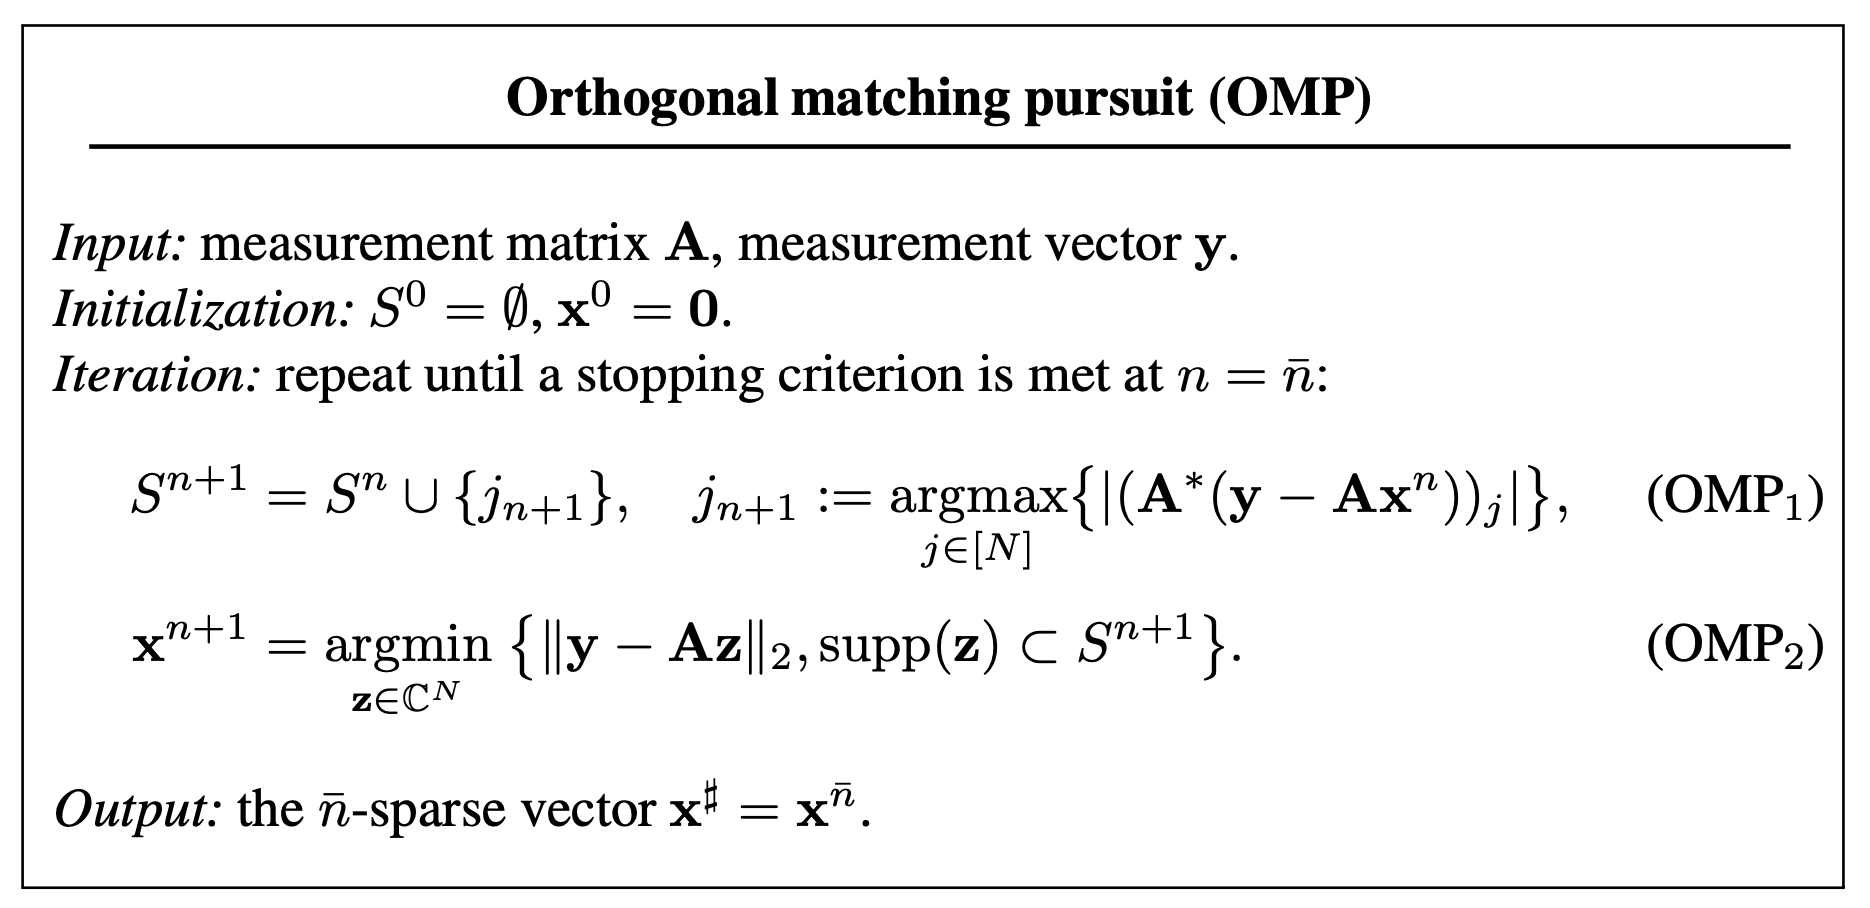
\includegraphics[width=\textwidth]{omp.png}
\end{figure}
下面的引理指出上述OMP算法中采用的策略$\underset{j \in[N]}{\operatorname{argmax}}\left\{\left|\left(\mathbf{A}^*\left(\mathbf{y}-\mathbf{A} \mathbf{x}^n\right)\right)_j\right|\right\}$
确实是一个好的贪心策略,确实满足了条件在欧氏距离下的最佳逼近。
\begin{lemma}
    令$\mathbf{A} \in \mathbb{C}^{m \times N}$是列归一化矩阵,给定的$S \subset[N]$,$\mathbf{v}$支撑在$S$上,并且
    $j \in[N]$,如果
    \begin{equation}
        \mathbf{w}:=\underset{\mathbf{z} \in \mathbb{C}^N}{\operatorname{argmin}}\left\{\|\mathbf{y}-\mathbf{A z}\|_2,\operatorname{supp}(\mathbf{z}) \subset S \cup\{j\}\right\}
    \end{equation}
    那么有
    \begin{equation}
        \|\mathbf{y}-\mathbf{A} \mathbf{w}\|_2^2 \leq\|\mathbf{y}-\mathbf{A v}\|_2^2-\left|\left(\mathbf{A}^*(\mathbf{y}-\mathbf{A} \mathbf{v})\right)_j\right|^2
    \end{equation}
\end{lemma}
\begin{proof}
任取$t \in \mathbb{C}$,形如$\mathbf{v}+t \mathbf{e}_j$的向量都支撑在$S \cup\{j\}$上,并且
\begin{equation}
    \|\mathbf{y}-\mathbf{A} \mathbf{w}\|_2^2 \leq \min _{t \in \mathbb{C}}\left\|\mathbf{y}-\mathbf{A}\left(\mathbf{v}+t \mathbf{e}_j\right)\right\|_2^2
\end{equation}
设$t=\rho e^{i \theta}$,有
\begin{equation}
    \begin{aligned}
    \left\|\mathbf{y}-\mathbf{A}\left(\mathbf{v}+t \mathbf{e}_j\right)\right\|_2^2 & =\left\|\mathbf{y}-\mathbf{A v}-t \mathbf{A} \mathbf{e}_j\right\|_2^2 \\
    & =\|\mathbf{y}-\mathbf{A v}\|_2^2+|t|^2\left\|\mathbf{A} \mathbf{e}_j\right\|_2^2-2 \operatorname{Re}\left(\bar{t}\left\langle\mathbf{y}-\mathbf{A v},\mathbf{A} \mathbf{e}_j\right\rangle\right) \\
    & =\|\mathbf{y}-\mathbf{A v}\|_2^2+\rho^2-2 \operatorname{Re}\left(\rho e^{-i \theta}\left(\mathbf{A}^*(\mathbf{y}-\mathbf{A v})\right)_j\right) \\
    & \geq\|\mathbf{y}-\mathbf{A v}\|_2^2+\rho^2-2 \rho\left|\left(\mathbf{A}^*(\mathbf{y}-\mathbf{A} \mathbf{v})\right)_j\right|
    \end{aligned}
\end{equation}
最后一式在$\rho=\left|\left(\mathbf{A}^*(\mathbf{y}-\mathbf{A} \mathbf{u})\right)_j\right|$时取最小,即
\begin{equation}
    \min _{t \in \mathbb{C}}\left\|\mathbf{y}-\mathbf{A}\left(\mathbf{v}+t \mathbf{e}_j\right)\right\|_2^2=\|\mathbf{y}-\mathbf{A v}\|_2^2-\left|\left(\mathbf{A}^*(\mathbf{y}-\mathbf{A} \mathbf{u})\right)_j\right|^2
\end{equation}
\end{proof}
正交匹配追踪算法有一个问题,一旦选择了不正确的索引,它就会保留下去,在$s$次迭代内没有办法修正。下面的CoSaMP算法增加了迭代次数,通过阈值的
引入增加了每次选取的个数,采用了更有意义的索引机制来减小陷入局部解的可能性。
设$\mathbf{z} \in \mathbb{C}^N$,令
\begin{equation}
    L_s(\mathbf{z}):=s\text{个最大绝对条目的索引集}
\end{equation}
\begin{equation}
    H_s(\mathbf{z}):=\mathbf{z}_{L_s(\mathbf{z})}
\end{equation}
其中非线性算子$H_s$称为$s$阶硬阈值运算符,它将保留绝对值最大的前$s$项,并将其他项置为0。\par
\begin{figure}[!htbp]
    \centering
    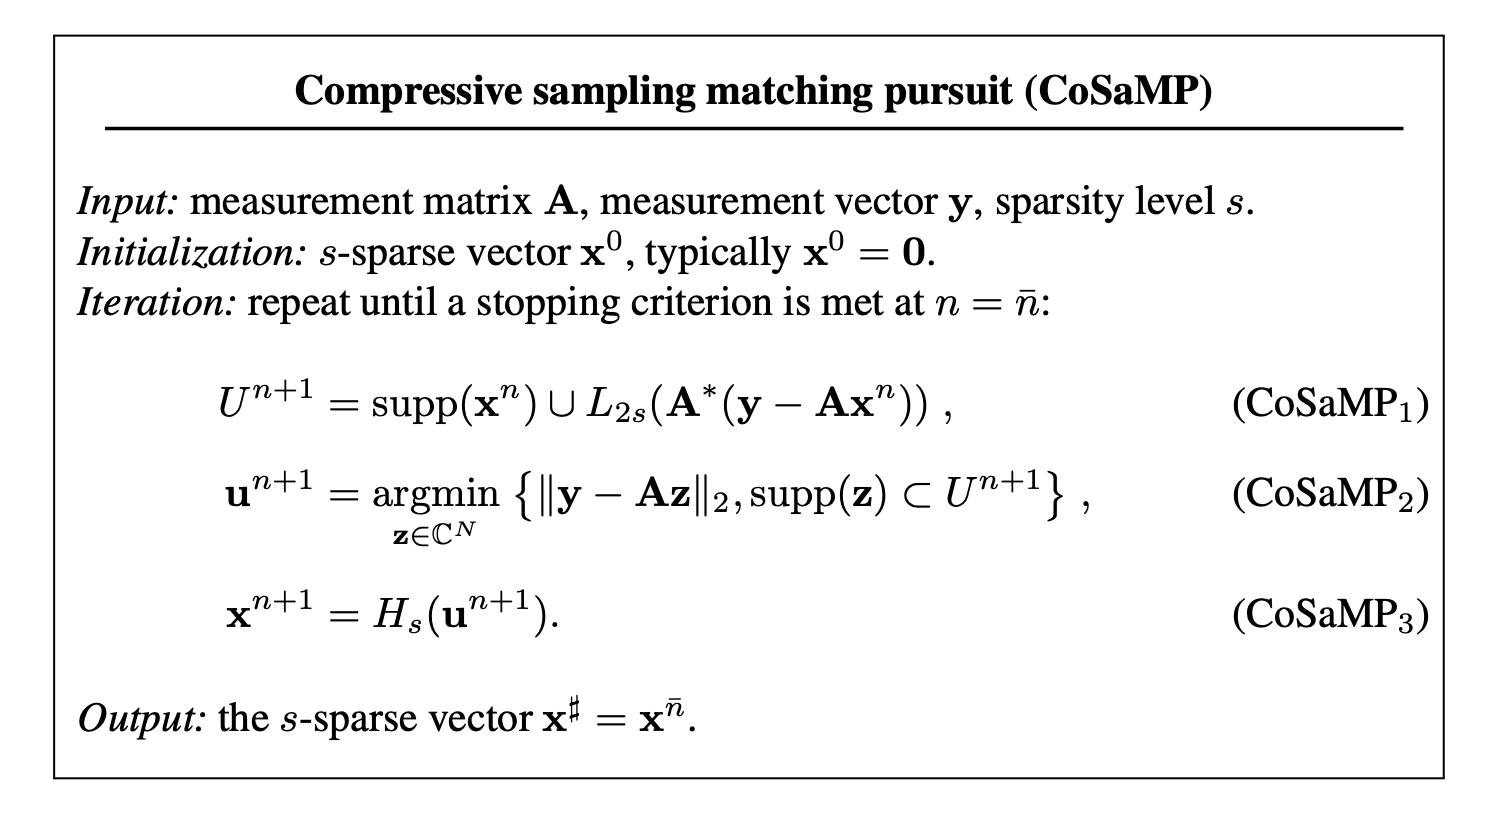
\includegraphics[width=\textwidth]{cosa.png}
\end{figure}






\section{小结}